% Source: Code/xband-radar-sim/docs/radar_simulation_technical.tex
% Description: Antenna gain pattern showing main lobe and sidelobes. The 3 dB beamwidth defines angular resolution.

\documentclass[border=4pt]{standalone}
\usepackage{algpseudocode}
\usepackage{amsmath,amssymb,amsfonts}
\usepackage[T1]{fontenc}
\usepackage{graphicx}
\usepackage{pgfplots}
\usepackage{tikz}
\usepackage{xcolor}
\pgfplotsset{compat=1.18}
\usetikzlibrary{arrows.meta,positioning,shapes.geometric,calc,patterns,decorations.pathmorphing,3d,angles,quotes}

\definecolor{radargreen}{RGB}{0,255,0}
\definecolor{raycolor}{RGB}{255,165,0}
\definecolor{targetcolor}{RGB}{255,0,0}
\definecolor{groundcolor}{RGB}{139,90,43}
\definecolor{skycolor}{RGB}{135,206,235}
\definecolor{beamcolor}{RGB}{255,255,0}


\begin{document}
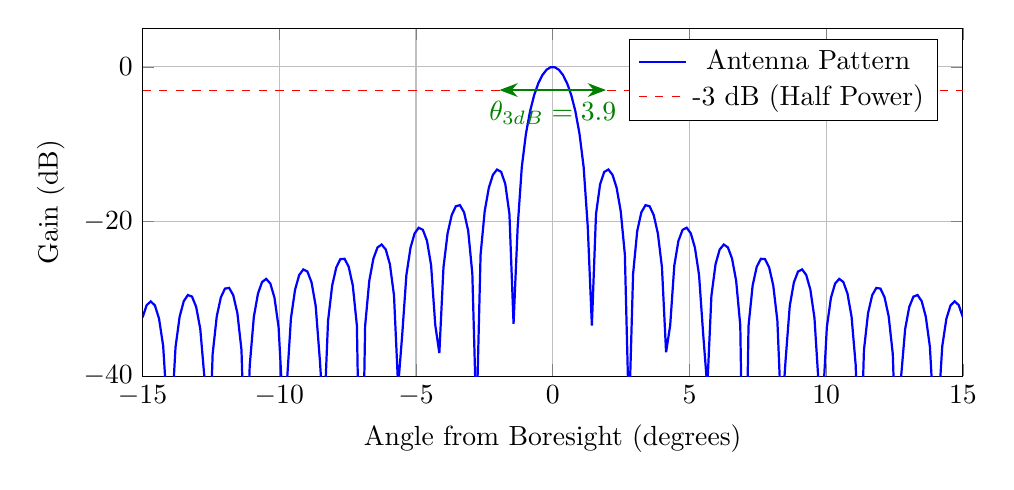
\begin{tikzpicture}
\begin{axis}[
    width=12cm, height=6cm,
    xlabel={Angle from Boresight (degrees)},
    ylabel={Gain (dB)},
    xmin=-15, xmax=15,
    ymin=-40, ymax=5,
    grid=both,
    legend pos=north east
]
    % Main lobe and sidelobes
    \addplot[thick, blue, domain=-15:15, samples=200] {
        20*log10(abs(sin(deg(pi*2.783*x/3.9))/(pi*2.783*x/3.9 + 0.0001)) + 0.0001)
    };
    \addlegendentry{Antenna Pattern}

    % 3dB line
    \addplot[dashed, red] coordinates {(-15,-3) (15,-3)};
    \addlegendentry{-3 dB (Half Power)}

    % Beamwidth annotation
    \draw[{Stealth}-{Stealth}, thick, green!50!black] (axis cs:-1.95,-3) -- (axis cs:1.95,-3);
    \node[green!50!black] at (axis cs:0,-6) {$\theta_{3dB} = 3.9°$};
\end{axis}
\end{tikzpicture}
\end{document}
